\documentclass[10pt,aspectratio=169]{beamer}

% ---------- Theme ----------
\usetheme{Madrid}
\usecolortheme{seahorse}
\setbeamertemplate{navigation symbols}{}
\setbeamertemplate{footline}[frame number]

% ---------- Packages ----------
\usepackage[utf8]{inputenc}
\usepackage{amsmath,amssymb,amsthm}
\usepackage{physics}      % for \bra, \ket, \expval, etc.
\usepackage{braket}
\usepackage{bm}
\usepackage{listings}
\usepackage{xcolor}
\usepackage{tikz}
\usetikzlibrary{quantikz}   % comment out if quantikz is not installed
\usepackage{hyperref}

% ---------- Code listing style ----------
\definecolor{codebg}{rgb}{0.96,0.96,0.98}
\definecolor{codekw}{rgb}{0.10,0.30,0.70}
\definecolor{codestr}{rgb}{0.55,0.20,0.20}
\definecolor{codecom}{rgb}{0.25,0.55,0.25}

\lstdefinestyle{pystyle}{
  language=Python,
  basicstyle=\ttfamily\scriptsize,
  keywordstyle=\color{codekw}\bfseries,
  stringstyle=\color{codestr},
  commentstyle=\color{codecom}\itshape,
  backgroundcolor=\color{codebg},
  frame=single,
  rulecolor=\color{black!20},
  showstringspaces=false,
  breaklines=true,
  numbers=left,
  numberstyle=\tiny\color{gray},
  tabsize=2,
  columns=fullflexible,
  upquote=true,
}
\lstset{style=pystyle}

% ---------- Title info ----------
\title[VQE \& Hartree--Fock]{Initialising Quantum States in VQE\\\large with a Hartree--Fock Reference}
\subtitle{Hybrid quantum--classical methods for eigenvalue problems}
\author{Notes for a quantum-computing / quantum-chemistry course}
\institute{}
\date{\today}

\begin{document}

% =========================================================
\begin{frame}
\titlepage
\end{frame}

% =========================================================
\begin{frame}{Outline}
\tableofcontents
\end{frame}

% =========================================================
\section{Motivation: eigenvalues on a quantum computer}

\begin{frame}{The problem we want to solve}
For an electronic Hamiltonian $\hat H$ acting on $N_q$ qubits we wish to obtain the lowest eigenvalue
\[
E_0 \;=\; \min_{\ket{\Psi}}\; \frac{\bra{\Psi}\hat H \ket{\Psi}}{\braket{\Psi}{\Psi}} .
\]

\textbf{Exact diagonalisation} scales as $\mathcal{O}(d^3)$ with $d=2^{N_q}$ — intractable for moderate molecules.

\smallskip
\textbf{Variational Quantum Eigensolver (VQE)} is a \emph{hybrid} algorithm:
\begin{itemize}
  \item A parameterised circuit $U(\bm{\theta})\ket{\Psi_0}$ prepares a trial state on the QPU.
  \item Expectation values $\expval{\hat H}{\Psi(\bm{\theta})}$ are measured on the QPU.
  \item A classical optimiser updates $\bm{\theta}$ to minimise the energy.
\end{itemize}
The variational principle guarantees $E(\bm{\theta}) \geq E_0$.
\end{frame}

% =========================================================
\begin{frame}{Why does the initial state matter?}
The ansatz wavefunction is
\[
\ket{\Psi(\bm{\theta})} \;=\; U(\bm{\theta})\,\ket{\Psi_0}.
\]
The \textbf{reference state} $\ket{\Psi_0}$ controls
\begin{itemize}
  \item the region of Hilbert space the optimiser can reach with reasonable circuit depth,
  \item the number of variational parameters needed for chemical accuracy,
  \item susceptibility to \emph{barren plateaus} and local minima.
\end{itemize}

\medskip
A bad reference (e.g.\ $\ket{0\cdots 0}$, the qubit vacuum) forces the ansatz to first build in the gross electronic structure before refining correlation.\\[2pt]
A good reference encodes the mean-field physics already, so $U(\bm{\theta})$ only has to add \emph{electron correlation}.

\medskip
$\Rightarrow$ The Hartree--Fock state is the natural starting point in quantum chemistry.
\end{frame}

% =========================================================
\section{Hartree--Fock in second quantisation}

\begin{frame}{Hartree--Fock recap}
The Hartree--Fock (HF) method approximates the many-electron wavefunction by a single Slater determinant
\[
\ket{\Phi_{\text{HF}}} \;=\; \frac{1}{\sqrt{N_e!}}\,
\det\!\left[\,\varphi_{i_1}(x_1)\cdots \varphi_{i_{N_e}}(x_{N_e})\,\right],
\]
where the spin-orbitals $\{\varphi_p\}$ are obtained by solving the Roothaan--Hall equations self-consistently.

\smallskip
In second quantisation, with creation operators $\hat a^{\dagger}_p$ acting on the Fock vacuum $\ket{\text{vac}}$,
\[
\boxed{\;\ket{\Phi_{\text{HF}}}\;=\; \prod_{p\,\in\, \text{occ}} \hat a^{\dagger}_p \;\ket{\text{vac}}\;}
\]
The occupied set $\text{occ}$ contains the $N_e$ lowest-energy spin-orbitals.
\end{frame}

% =========================================================
\begin{frame}{From fermions to qubits}
A qubit can represent the occupation of one spin-orbital:
\[
\ket{0}_p \;\leftrightarrow\; \text{orbital } p \text{ empty}, \qquad
\ket{1}_p \;\leftrightarrow\; \text{orbital } p \text{ occupied}.
\]

We need a transformation that maps fermionic operators (with antisymmetry) onto qubit operators (Pauli strings). Standard choices:
\begin{itemize}
  \item \textbf{Jordan--Wigner (JW)} --- simple, local in occupation but non-local in parity strings.
  \item \textbf{Parity} mapping --- swaps the locality trade-off.
  \item \textbf{Bravyi--Kitaev (BK)} --- $\mathcal{O}(\log N)$ locality in both.
\end{itemize}

\smallskip
\textbf{Jordan--Wigner:}
\[
\hat a^{\dagger}_p \;=\; \left(\prod_{q<p} Z_q\right) \frac{X_p - i Y_p}{2}.
\]

Crucially, under JW the HF Slater determinant becomes a single computational-basis state.
\end{frame}

% =========================================================
\begin{frame}{The HF state under Jordan--Wigner}
With JW ordering (spin-orbitals indexed $0,1,\ldots,M-1$, occupied first),
\[
\ket{\Phi_{\text{HF}}}_{\text{JW}}
\;=\;
\underbrace{\ket{1}\ket{1}\cdots\ket{1}}_{N_e\ \text{occupied}}
\;
\underbrace{\ket{0}\ket{0}\cdots\ket{0}}_{M-N_e\ \text{virtual}}.
\]

\textbf{This is a product state!} It is prepared from $\ket{0}^{\otimes M}$ by applying $X$ gates on the first $N_e$ qubits:

\begin{center}
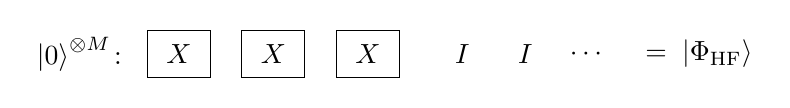
\begin{tikzpicture}
\node[draw, rectangle, minimum width=0.8cm, minimum height=0.6cm] (x1) at (0,0) {$X$};
\node[draw, rectangle, minimum width=0.8cm, minimum height=0.6cm] (x2) at (1.2,0) {$X$};
\node[draw, rectangle, minimum width=0.8cm, minimum height=0.6cm] (x3) at (2.4,0) {$X$};
\node at (3.6,0) {$I$};
\node at (4.4,0) {$I$};
\node at (5.2,0) {$\cdots$};
\node[anchor=east] at (-0.6,0) {$\ket{0}^{\otimes M}\!:$};
\node[anchor=west] at (5.8,0) {$=\;\ket{\Phi_{\text{HF}}}$};
\end{tikzpicture}
\end{center}

\smallskip
For $\mathrm{H}_2$ in a minimal basis (STO-3G):
\[
M = 4\ \text{spin-orbitals},\quad N_e = 2 \;\Longrightarrow\; \ket{\Phi_{\text{HF}}} = \ket{1100}.
\]
\end{frame}

% =========================================================
\section{Building the reference in code}

\begin{frame}[fragile]{A bare-bones HF initialiser in Qiskit}
\textbf{Goal:} prepare $\ket{1100}$ for H$_2$ with a hand-rolled circuit.
\begin{lstlisting}
from qiskit import QuantumCircuit, QuantumRegister

def hartree_fock_jw(n_spin_orbitals, n_electrons):
    """
    Prepare a Hartree-Fock reference under Jordan-Wigner mapping.
    Occupied orbitals are assumed to be the lowest n_electrons indices.
    """
    qr = QuantumRegister(n_spin_orbitals, name="q")
    qc = QuantumCircuit(qr, name="HF")
    for i in range(n_electrons):
        qc.x(qr[i])           # flip |0> -> |1> on occupied orbitals
    return qc

hf_circuit = hartree_fock_jw(n_spin_orbitals=4, n_electrons=2)
print(hf_circuit)
\end{lstlisting}

\smallskip
\textbf{Output (schematic):}
\begin{verbatim}
q_0: ─X─
q_1: ─X─
q_2: ───
q_3: ───
\end{verbatim}
That is the entire HF state preparation under JW: $N_e$ Pauli-$X$ gates.
\end{frame}

% =========================================================
\begin{frame}[fragile]{Using Qiskit Nature's built-in HF initial state}
For production work, use the library — it handles JW, parity (with two-qubit reduction), and BK consistently.
\begin{lstlisting}
from qiskit_nature.second_q.circuit.library import HartreeFock
from qiskit_nature.second_q.mappers import JordanWignerMapper

mapper = JordanWignerMapper()

hf_init = HartreeFock(
    num_spatial_orbitals = 2,    # H2 in STO-3G has 2 spatial orbitals
    num_particles        = (1, 1),  # (alpha, beta) electrons
    qubit_mapper         = mapper,
)

print(hf_init.draw())
# Equivalent to manually applying X on the occupied spin-orbital qubits.
\end{lstlisting}

\smallskip
Switching mapper $=$ switching the bit-pattern that represents HF; the library does the bookkeeping for you.
\end{frame}

% =========================================================
\begin{frame}[fragile]{Full pipeline: HF $\to$ UCCSD $\to$ VQE for H$_2$}
\begin{lstlisting}
from qiskit_nature.second_q.drivers import PySCFDriver
from qiskit_nature.second_q.mappers import JordanWignerMapper
from qiskit_nature.second_q.circuit.library import HartreeFock, UCCSD
from qiskit_algorithms import VQE
from qiskit_algorithms.optimizers import SLSQP
from qiskit.primitives import Estimator

# 1. Classical electronic-structure problem (PySCF backend)
driver  = PySCFDriver(atom="H 0 0 0; H 0 0 0.735", basis="sto3g")
problem = driver.run()
hamiltonian = problem.hamiltonian.second_q_op()

# 2. Map fermions -> qubits
mapper      = JordanWignerMapper()
qubit_op    = mapper.map(hamiltonian)

# 3. Hartree-Fock initial state
hf_state = HartreeFock(
    num_spatial_orbitals = problem.num_spatial_orbitals,
    num_particles        = problem.num_particles,
    qubit_mapper         = mapper,
)

# 4. UCCSD ansatz built ON TOP OF the HF reference
ansatz = UCCSD(
    num_spatial_orbitals = problem.num_spatial_orbitals,
    num_particles        = problem.num_particles,
    qubit_mapper         = mapper,
    initial_state        = hf_state,    # <-- the key line
)

# 5. Run VQE
vqe    = VQE(Estimator(), ansatz, SLSQP(maxiter=200))
result = vqe.compute_minimum_eigenvalue(qubit_op)
print("VQE electronic energy:", result.eigenvalue.real)
\end{lstlisting}
\end{frame}

% =========================================================
\begin{frame}{What the ansatz actually does}
The unitary coupled-cluster singles-and-doubles (UCCSD) ansatz reads
\[
\ket{\Psi(\bm\theta)} \;=\; e^{\hat T(\bm\theta) - \hat T^{\dagger}(\bm\theta)} \,\ket{\Phi_{\text{HF}}},
\qquad
\hat T = \hat T_1 + \hat T_2,
\]
\[
\hat T_1 = \sum_{i\in\text{occ}, a\in\text{virt}} \theta_i^{a}\, \hat a^{\dagger}_a \hat a_i,
\quad
\hat T_2 = \tfrac14 \sum_{ij,ab} \theta_{ij}^{ab}\, \hat a^{\dagger}_a \hat a^{\dagger}_b \hat a_j \hat a_i.
\]

Two crucial properties when starting from $\ket{\Phi_{\text{HF}}}$:
\begin{itemize}
  \item At $\bm\theta = 0$, $\ket{\Psi(0)} = \ket{\Phi_{\text{HF}}}$, so the optimiser starts at the HF energy — a known, sensible baseline.
  \item Each excitation operator $\hat a^{\dagger}_a \hat a_i$ promotes an electron from an occupied to a virtual orbital, i.e.\ it generates correlation \emph{on top of} HF.
\end{itemize}
\end{frame}

% =========================================================
\section{Beyond simple HF: subtleties and alternatives}

\begin{frame}{Different mappings change the bit pattern}
Same physical state, different representation on the qubits:
\begin{center}
\begin{tabular}{lll}
\hline
Mapping & H$_2$ HF state & \# qubits \\
\hline
Jordan--Wigner       & $\ket{1100}$        & 4 \\
Parity               & $\ket{0110}$        & 4 \\
Parity + Z$_2$ symm. & $\ket{01}$          & 2 \\
Bravyi--Kitaev       & $\ket{1110}$        & 4 \\
\hline
\end{tabular}
\end{center}
\smallskip
Lesson: \emph{never} hard-code an HF bit pattern. Always derive it from the mapper and the orbital ordering, or rely on a library helper.

\smallskip
The two-qubit reduction (parity mapping $+$ $Z_2$ symmetries) is a particularly useful trick for small molecules — H$_2$ in STO-3G drops from 4 to 2 qubits.
\end{frame}

% =========================================================
\begin{frame}{When HF is not enough}
HF is a \emph{mean-field} reference. It breaks down for systems with strong static correlation:
\begin{itemize}
  \item stretched bonds (H$_2$ at large $R$, N$_2$ dissociation),
  \item transition-metal complexes with near-degenerate $d$-orbitals,
  \item open-shell singlets, conical intersections.
\end{itemize}

\smallskip
Possible remedies as initial states for VQE:
\begin{itemize}
  \item \textbf{Multi-reference HF} or \textbf{CASSCF} → linear combination of Slater determinants, prepared with an entangling circuit.
  \item \textbf{Symmetry-broken HF (UHF)} → cheaper but loses spin symmetry.
  \item \textbf{Adaptive ansätze} (ADAPT-VQE) → grow the ansatz operator-by-operator starting from HF; partly compensates for a poor reference.
\end{itemize}

A useful diagnostic: if $|1 - \langle S^2\rangle / S(S+1)|$ is large at $\bm\theta = 0$, HF is a poor starting point.
\end{frame}

% =========================================================
\begin{frame}[fragile]{Preparing a multi-determinant reference}
A two-determinant reference, e.g.\
\(\ket{\Psi_0} = \cos\alpha\,\ket{\Phi_{\text{HF}}} + \sin\alpha\,\ket{\Phi^{ab}_{ij}}\),
needs one entangling block on top of the X-gate layer.

\smallskip
Conceptually:
\begin{lstlisting}
from qiskit import QuantumCircuit
from numpy import pi

def two_det_reference(alpha):
    qc = QuantumCircuit(4)
    # HF part: |1100>
    qc.x(0); qc.x(1)
    # Rotate amplitude into the doubly-excited determinant |0011>
    qc.ry(2*alpha, 0)
    qc.cx(0, 2)
    qc.cx(1, 3)
    qc.x(0); qc.x(1)
    return qc

print(two_det_reference(pi/8).draw())
\end{lstlisting}

\smallskip
The pattern generalises: any configuration-interaction reference can be prepared with $\mathcal{O}(\text{\# determinants})$ controlled rotations under JW.
\end{frame}

% =========================================================
\section{Summary}

\begin{frame}{Take-home messages}
\begin{itemize}
  \item VQE turns an eigenvalue problem into an optimisation over circuit parameters — \emph{the starting point of that optimisation matters}.
  \item The Hartree--Fock state is the natural and cheap reference inherited from classical quantum chemistry.
  \item Under Jordan--Wigner the HF state is a single product state $\ket{1\cdots1\,0\cdots0}$, prepared by $N_e$ Pauli-$X$ gates.
  \item Different fermion-to-qubit mappings give different HF bit patterns — let a library compute them for you.
  \item For strongly correlated systems, supplement HF with a small entangling layer (multi-determinant reference) or use an adaptive ansatz.
\end{itemize}

\bigskip
\textbf{Suggested follow-ups:}
\begin{itemize}
  \item Hardware-efficient ansätze and their initialisation pitfalls (barren plateaus).
  \item Symmetry-preserving ansätze (number, $S^2$, $S_z$ conservation).
  \item Reading: McArdle \emph{et al.}, \emph{Rev. Mod. Phys.} 92, 015003 (2020); Tilly \emph{et al.}, \emph{Phys. Rep.} 986, 1 (2022).
\end{itemize}
\end{frame}

% =========================================================
\begin{frame}{}
\centering
\Large Questions and discussion
\end{frame}

\end{document}
